%=========================================================
\chapter{Contexto}
\label{cap:reqUsr}

	En este capítulo se definen conceptos referentes a la Administración y Gestión de proyectos, sin embargo solo nos enfocaremos en los que tienen relación con el proyecto que se esta realizando. Ademas se habla sobre algunas Técnicas utilizadas en la toma de decisiones, que fueron consideradas para dar solución a la problematica que se pretende resolver con este Sistema.
%---------------------------------------------------------
\section{Proyecto}	
Un proyecto es un esfuerzo temporal que se lleva a cabo para crear un producto, servicio o resultado único, determinado por un presupuesto y programa. La naturaleza temporal de los proyectos implica que un proyecto tiene un principio y un final definidos por su tamaño y complejidad. Otro aspecto es que tiene un objetivo claro que establece lo que se logrará. Además de que este puede incluir también una declaración de los beneficios o resultados esperados que se lograrán a partir de la implementación de los objetivos del mismo.\cite{J. Gido P.}
%---------------------------------------------------------
\section{Ciclo de vida de un proyecto }	
El ciclo de vida de un proyecto es la serie de fases por las que atraviesa un proyecto desde su inicio hasta su cierre. Las fases son generalmente secuenciales y sus nombres y números se determinan en función de las necesidades de gestión y control de la organización u organizaciones que participan en el proyecto. El ciclo de vida de un proyecto no debe confundirse con los grupos de procesos de la dirección de proyectos, ya que los procesos de un grupo de procesos consisten en actividades que pueden realizarse y repetirse dentro de cada fase de un proyecto.\cite{PMBOK}  

La Guía del PMBOK en su 5ta edición dice que todos los proyectos pueden configurarse dentro de la siguiente estructura genérica de ciclo de vida:

\begin{itemize}
\item Planificación
\item Organización y preparación
\item Monitoreo
\item Cierre del proyecto.
\end{itemize}
Esta perspectiva general puede proporcionar un marco de referencia común para comparar proyectos, incluso si son de naturaleza diferente. La siguiente grafica perteneciente al PMBOK en su 5ta edición da un ejemplo de lo anteriormente mencionado. 
\begin{figure}[htbp!]
	\begin{center}
		\fbox{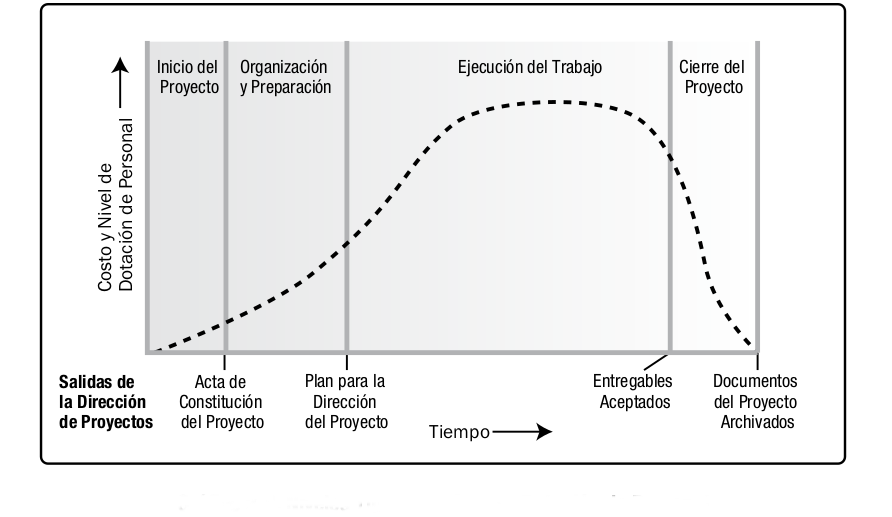
\includegraphics[width=.6\textwidth]{images/ciclodevidadeunproyecto}}
		\caption{Ciclo de vida de un proyecto de software.}
		\label{fig:ciclodevidadeunproyecto}
	\end{center}
\end{figure}


%---------------------------------------------------------
\section{Información del proyecto}	

A lo largo del ciclo de vida del proyecto, se recopila, analiza, transforma y distribuye a los miembros del equipo del proyecto y a otros interesados una cantidad significativa de datos e información en diversos formatos. Los datos del proyecto se recopilan y analizan de forma continua durante el transcurso del proyecto. 
\newline
Dentro de ellos podemos mencionar:
\begin{itemize}
\item Datos de desempeño del trabajo: Son las observaciones y mediciones directas identificadas durante las actividades ejecutadas para llevar a cabo el trabajo del proyecto. Entre los ejemplos se incluyen el porcentaje de trabajo físicamente terminado, las medidas de desempeño técnico y de calidad, las fechas de comienzo y finalización de las actividades planificadas, el número de solicitudes de cambio, el número de defectos, los costos reales, las duraciones reales, etc. 
\item Información de desempeño del trabajo: Son los datos de desempeño recopilados de varios procesos de control, analizados en contexto e integrados en base a las relaciones entre las áreas. Algunos ejemplos de información sobre el desempeño del trabajo son el estado de los entregables, el estado de implementación de las solicitudes de cambio y las estimaciones hasta la conclusión previstas.
\item Informes de desempeño del trabajo: Constituyen la representación física o electrónica de la información de desempeño del trabajo recogida en documentos del proyecto para la toma de decisiones, el planteamiento de incidentes, el emprendimiento de acciones y la generación de conocimiento. Entre los ejemplos se pueden citar los informes de estado, los memorandos, las justificaciones, las notas informativas, los cuadros de mando electrónicos, las recomendaciones y las actualizaciones.\cite{R. Lopez.}\cite{PMBOK}
\end{itemize}

%---------------------------------------------------------
\section{Proceso de un proyecto}	
Un proceso es un conjunto de acciones y actividades, relacionadas entre sí, que se realizan para crear un producto, resultado o servicio predefinido. Cada proceso se caracteriza por sus entradas, por las herramientas y técnicas que se pueden aplicar y por las salidas que se obtienen.\cite{PMBOK}
\newline
Una vez definido lo que es un proyecto y viendo las etapas del mismo. Podemos introducirnos a lo que es la Administración y Gestión de proyecto. 
%---------------------------------------------------------
\section{Administración de proyectos}
La administración de proyectos se define como: la planeación, organización, coordinación, dirección y control de los recursos para lograr el objetivo del proyecto, en el menor tiempo posible y mínimo de errores. \cite{J. Gido P.}\cite{PMBOK}\cite{Adproyectos}Por otra parte la administración de proyectos comprende los pasos siguientes:

Establecer el objetivo del proyecto. El objetivo debe ser acordado entre el cliente y la organización ejecutora del proyecto. 
\begin{itemize}
 

\item Definir el alcance. Debe prepararse un documento de alcance del proyecto que incluya los requerimientos del cliente, defina las tareas de trabajo o elementos principales, y determinar una lista de entregables y los criterios de aceptación correspondientes que se pueden utilizar para verificar que el trabajo y los entregables cumplen con las especificaciones. 

 

\item  Crear una estructura de división del trabajo. Subdivida el alcance del proyecto en partes o paquetes de trabajo. Aunque los proyectos pueden parecer abrumadores cuando se ven como un todo, una forma de salir victorioso incluso de la tarea más monumental es dividirla en componentes pequeños. Una estructura de división del trabajo (EDT) es una descomposición jerárquica del alcance del proyecto en elementos de trabajo que ejecutará el equipo del proyecto que producirá los entregables respectivos.  

 

\item Asignar responsabilidades. Debe identificarse la persona u organización responsable de cada elemento de trabajo en la estructura de la división del trabajo. De esta manera el equipo del proyecto estará informado de quién es la persona responsable y de los resultados del desempeño de cada paquete de trabajo y cualquier entregable relacionado.  

 

\item Definir las actividades específicas. Revisar cada paquete de trabajo en la estructura de división del trabajo y elaborar una lista de las actividades detalladas que se deben realizar para cada paquete y para producir todos los entregables requeridos. 

 

Establecer la secuencia de las actividades. 

 

\item Estimar los recursos de las actividades. Determine los tipos de recursos, como las habilidades necesarias para realizar cada actividad, así como la cantidad que se requerirá de cada recurso. Los recursos incluyen las personas, materiales, equipos, etcétera, que se necesiten para realizar cada actividad. Las estimaciones de los recursos deben tener en cuenta la disponibilidad de cada tipo de recurso, ya sea interno o externo (como los subcontratistas), y la cantidad disponible durante la duración del proyecto. Designe a una persona específica para que se encargue de cada actividad. 

 

\item Estimar la duración de las actividades. Haga una estimación del tiempo que tomará completar cada actividad, con base en los recursos que se aplicarán. 

 

\item Estimar los costos de la actividad. Los costos de una actividad deben basarse en los tipos y las cantidades de los recursos estimados para cada actividad, así como en la tasa de costo de mano de obra apropiada o el costo unitario de cada tipo de recurso. 

 

\item Determinar el presupuesto. El presupuesto total del proyecto se puede desarrollar al añadir las estimaciones de costos para cada actividad. Así mismo, los presupuestos para cada paquete de trabajo en la estructura de la división del trabajo se determinan al añadir los costos estimados de las actividades detalladas para cada paquete de trabajo. Otros costos, como los administrativos del proyecto o de la organización y los costos indirectos o generales, también se deben incluir en el presupuesto y asignarse debidamente a cada actividad o paquete de trabajo. Una vez que se determina el presupuesto total para el proyecto en general o para cada paquete de trabajo, se debe desarrollar un presupuesto en etapas para distribuir los fondos a lo largo de la duración del proyecto o paquete de trabajo, con base en las fechas esperadas de inicio y terminación de cada actividad estipuladas en el programa del proyecto.\cite{PMBOK}
\end{itemize}
%---------------------------------------------------------
\section{Dirección de proyectos}

A diferencia de la Administración, la dirección de proyectos es la aplicación de conocimientos, habilidades, herramientas y técnicas a las actividades del proyecto para cumplir con los requisitos del mismo. Esta aplicación de conocimientos requiere de la realización eficaz de los procesos de dirección de proyectos. Además de requerir que cada proceso del proyecto esté alineado y conectado de manera adecuada con los demás procesos, a fin de facilitar la coordinación. Generalmente las acciones tomadas durante la ejecución de un proceso afectan a ese proceso y a otros procesos relacionados.\cite{PMBOK}
\newline
La Guía del PMBOK describe que los procesos de la dirección de proyectos se agrupan en cinco categorías conocidas como Grupos de Procesos de la Dirección de Proyectos (o Grupos de Procesos): 
\begin{itemize}
\item Grupo de Procesos de Inicio. Aquellos procesos realizados para definir un nuevo proyecto o nueva fase de un proyecto existente al obtener la autorización para iniciar el proyecto o fase. 

\item Grupo de Procesos de Planificación. Aquellos procesos requeridos para establecer el alcance del proyecto, refinar los objetivos y definir el curso de acción requerido para alcanzar los objetivos propuestos del proyecto. 

\item Grupo de Procesos de Ejecución. Aquellos procesos realizados para completar el trabajo definido en el plan para la dirección del proyecto a fin de satisfacer las especificaciones del mismo. 

\item Grupo de Procesos de Monitoreo y Control. Aquellos procesos requeridos para rastrear, revisar y regular el progreso y el desempeño del proyecto, para identificar áreas en las que el plan requiera cambios y para iniciar los cambios correspondientes. 

\item Grupo de Procesos de Cierre. Aquellos procesos realizados para finalizar todas las actividades a través de todos los Grupos de Procesos, a fin de cerrar formalmente el proyecto o una fase del mismo.\cite{PMBOK}
\end{itemize}
 
Por otra parte, Frank Tsui divide estos mismos procesos de la siguiente forma: 

Planeación, Organización, Monitoreo y Ajuste, siendo este último el que se encargue de definir de nuevo la planeación del proyecto, haciendo como su nombre lo dice un reajuste al proyecto.\cite{SistemaGestor}
%---------------------------------------------------------
\section{Líder de proyecto}
Su misión es la de dirigir y coordinar los proyectos de desarrollo y mantenimiento de las aplicaciones de un área de la empresa, supervisando las funciones y los recursos de análisis funcional, técnico y programación, con el fin de satisfacer las necesidades de los usuarios y asegurando la adecuada explotación de las aplicaciones.\cite{LideresProyectos} 

Lo que se requiere para desempeñar un puesto de estas características son amplios conocimientos en distintas áreas o entornos de trabajo.
\newline \newline
\textbf {Competencias Blandas} 

\begin{itemize}
\item Orientación al logro de objetivos 

\item Desarrollo y Dirección de recursos 

\item Confianza en sí mismo y en el equipo 

\item Manejo de conflictos (resistencia al cambio) 

\item Capacidad de análisis (estructurada en lo referente a sus funciones y abierta al conocimiento y aplicaciones de nuevas tecnologías) 

\item Decisión 

\item Capacidad de comunicación 

\item Capacidad para trabajar bajo presión 
\end{itemize}

\textbf {Competencias Técnicas} 

\begin{itemize}
\item Formación Profesional Universitaria (Sistemas/Administración de Empresas/Cs. Económicas) 

\item Metodologías de desarrollo e implementación de proyectos 

\item Gestión de Recursos Humanos

\end{itemize}
%---------------------------------------------------------
\section{Toma de decisiones}
La toma de decisiones es el proceso mediante el cual la persona debe escoger entre dos o más alternativas. Tomar decisiones es el resultado de un proceso en el cual es importante conocer la manera cómo el agente que las toma consigue expresar sus preferencias.\cite{TomaDecisiones} 

Para los administradores de proyectos, el proceso de toma de decisión es sin duda una de las mayores responsabilidades. La toma de decisiones en una organización se circunscribe a una serie de personas que están apoyando el mismo proyecto. Debemos empezar por hacer una selección de decisiones y esta selección es una de las tareas de gran trascendencia. 
\newline \newline
Los administradores de proyectos consideran a veces la toma de decisiones como su trabajo principal, porque constantemente tienen que decidir lo que debe hacerse, quién ha de hacerlo, cuándo y dónde, y en ocasiones hasta cómo se hará. Sin embargo, la toma de decisiones sólo es un paso de la planeación, incluso cuando se hace con rapidez y dedicándole poca atención o cuando influye sobre la acción sólo durante unos minutos. 
\newline \newline
La toma de decisiones en una organización invade cuatro funciones administrativas que son: planeación, organización, dirección y control.\cite{TecnicasDecisiones}
%---------------------------------------------------------
\subsection{Planeación} 

Selección de misiones y objetivos, así como de las acciones para cumplirlas. Esto implica “Toma de decisión”.  

\begin{itemize}
\item ¿Cuáles son los objetivos de la organización, a largo plazo? 

\item ¿Qué estrategias son mejores para lograr este objetivo? 

\item ¿Cuáles deben ser los objetivos a corto plazo? 

\item ¿Cuán altas deben ser las metas individuales?

\end{itemize}
%---------------------------------------------------------
\subsection{Organización} 

Establecimiento de la estructura de la organización y cómo se desempeñan los individuos dentro de ella. 

\begin{itemize}
\item ¿Cómo deben diseñarse los puestos? 

\item ¿Quién está mejor calificado para ocupar un puesto vacante? 

\item ¿Cuándo debe una organización instrumentar una estructura diferente

\end{itemize}

%---------------------------------------------------------
\subsection{Dirección} 

Esta función requiere que los administradores influyan en los individuos para el cumplimiento de las metas organizacionales y grupales. 

\begin{itemize}
\item ¿Cómo manejo a un grupo de trabajadores que parecen tener una motivación baja? 

\item ¿Cuál es el estilo de liderazgo más eficaz para una situación dada? 

\item ¿Cómo afectará un cambio específico a la productividad del trabajador? 

\item ¿Cuándo es adecuado estimular el conflicto? 

\end{itemize}
%---------------------------------------------------------
\subsection{Control} 

Es la medición y corrección del desempeño individual y organizacional de manera tal que se puedan lograr los planes.

\begin{itemize}
\item ¿Qué actividades en la organización necesitan ser controladas? 

\item ¿Cómo deben controlarse estas actividades? 

\item ¿Cuándo es significativa una desviación en el desempeño? 

\item ¿Cuándo la organización está desempeñándose de manera efectiva? 

\end{itemize}

%---------------------------------------------------------
\section{Características de la decisión} 

Es la medición y corrección del desempeño individual y organizacional de manera tal que se puedan lograr los planes.

\begin{itemize}
\item Efectos futuros  

Tiene que ver con la medida en que los compromisos relacionados con la decisión afectarán el futuro. Una decisión que tiene una influencia a largo plazo puede ser considerada una decisión de alto nivel, mientras que una decisión con efectos a corto plazo puede ser tomada a un nivel muy inferior. 
\item Reversibilidad 

 Se refiere a la velocidad con que una decisión puede revertirse y la dificultad que implica hacer este cambio. Si revertir es difícil, se recomienda tomar la decisión a un nivel alto; pero si revertir es fácil, se requiere tomar la decisión a un nivel bajo. 
 
 \item Impacto 

Esta característica se refiere a la medida en que otras áreas o actividades se ven afectadas. Si el impacto es extensivo, es indicado tomar la decisión a un nivel alto; un impacto único se asocia con una decisión tomada a un nivel bajo. 

\item Calidad  

Este factor se refiere a las relaciones laborales, valores éticos, consideraciones legales, principios básicos de conducta, imagen de la compañía, etc. Si muchos de estos factores están involucrados, se requiere tomar la decisión a un nivel alto; si solo algunos factores son relevantes, se recomienda tomar la decisión a un nivel bajo. 

\item Periodicidad 

Este elemento responde a la pregunta de si una decisión se toma frecuente o excepcionalmente. Una decisión excepcional es una decisión de alto nivel, mientras que una decisión que se toma frecuentemente es una decisión de nivel bajo.\cite{TecnicasDecisiones}

\end{itemize}


%---------------------------------------------------------
\section{Técnicas normalmente utilizadas en la toma de decisiones.} 
\subsection{Minería de datos} 
La minería de datos se puede definir como un conjunto de técnicas y herramientas, que permiten la exploración de bases de datos, con el objetivo de encontrar patrones o reglas que expliquen los modelos de negocio. 

\subsection*{Minería de datos para la toma de decisiones} 

El uso de la minería de datos como soporte a decisiones en los negocios es más que aplicar redes neuronales o árboles de decisión sobre los datos  por un lado está el descubrimiento del conocimiento en la base de datos y por otro lado están las técnicas estadísticas como el reconocimiento de patrones y algoritmos de aprendizaje entre otros.\cite{R. Lopez.}

Los datos tal y como se almacenan en las bases de datos no suelen proporcionar beneficios directos , el valor está en la información que podamos extraer de ellos , que es la información que nos ayuda en la toma de decisiones o mejorar la comprensión del entorno que nos rodea, como puede ser la comprobación de que todo va bien , analizar diferentes aspectos de la evolución de la empresa , comparar información en diferentes periodos de tiempo , comparar resultados con previsiones, para ello se tienen que definir medidas cualitativas para los patrones obtenidos como son la precisión , utilidad y beneficio obtenido. \cite{R. Lopez.}

La implementación de procesos de minería de datos a través de la aplicación de técnicas estadísticas avanzadas y nuevos métodos de extracción de conocimiento en grandes bases de datos se pueden determinar las características contables de empresas más rentables al igual que el perfil de sus clientes, es necesario, por tanto, un análisis exploratorio profundo de la base de datos y el empleo de métodos que hagan que dichos modelos sean menos sensibles a los casos estadísticos. La mayoría de los trabajos de minería de datos están orientados al data warehouse, arquitectura de algoritmos, herramientas y técnicas utilizadas para agrupar los datos provenientes de múltiples bases de datos u otras fuentes de información en un repositorio común sobre el cual de harán consultas y análisis, se esta forma se consigue orientar los datos hacia el negocio.\cite{R. Lopez.}\cite{MineriaDatos}

Algunas técnicas que ayudan a la resolución de problemas de la organización basándose en los datos que se poseen son:
\begin{itemize}
\item Razonamiento estadístico, se utilizan para datos del pasado y la estadística tiene un peso significativo 

\item Procesamiento paralelo, para agilizar el procesamiento de consultas 

\item Apoyo a la toma de decisiones, basados en la teoría de la decisión 

\item Aprendizaje automático, consiste en aprender reglas a partir de los datos, aprender experiencias del pasado con respecto a alguna medida de rendimiento.\cite{R. Lopez.}
\end{itemize}


\subsection{Reconocimiento de patrones en la toma de decisiones } 

El reconocimiento de patrones es la ciencia que se ocupa de los procesos sobre ingeniería, computación y matemáticas relacionados con objetos físicos o abstractos, con el propósito de extraer información que permita establecer propiedades de entre conjuntos de dichos objetos. \cite{TomaDecisiones}

El reconocimiento de patrones es una técnica de la inteligencia artificial y es empleado por tecnologías como el procesamiento del lenguaje natural y la visión computacional.\cite{TecnicasDecisiones} 

El reconocimiento de patrones se apoya de otras técnicas de la IA como: 
\begin{itemize}
\item Lógica Difusa 

\item Minería de Datos 

\item Redes Neuronales 
\end{itemize} 

Además, se apoya en técnicas de otras ciencias
\begin{itemize}
\item Estadística 

\item Geometría 

\item Teoría de Lenguajes 

\item Lógica Simbólica 

\item Entre otras 
\end{itemize}


%---------------------------------------------------------
\section{Problemas identificados } 
Los problemas que se describen a continuación son los mas comunes en el desarrollo de proyectos de software.Es importante destacar que solo nos enfocaremos en los que para nosostros tienen mayor prioridad. 
\begin{itemize}
\item Mala planificación
Más vale tomar el tiempo necesario para hacer una excelente planificación al inicio de un proyecto, que una buena planificación al final. 
\begin{itemize}
\item Tiempo 
\begin{itemize}
\item Retrasos  

La planificación de tiempo no depende solo de la duración propuesta para un proyecto, influyen otras variables como son la complejidad de las tareas a realizar, equipo disponible para trabajar, y el presupuesto para llevarlo a cabo, un error común es pensar solo en uno de ellos lo cual conlleva a un fracaso al final. 
\end{itemize}

\item Recursos  

Se refiere a todo aquello que se ve involucrado en la realización del proyecto (dinero, equipo, etc.). Una mala decisión de principio conlleva a que un proyecto fracase. 
\item Riesgos 

\item Estimaciones erróneas 

Va muy relacionado con los recursos, pues cuando se tiene muy poca experiencia en la gestión de proyecto es normal que se hagan estimaciones erróneas, en recursos (material, equipo, o personal), así como en presupuesto. 
\end{itemize}
\item El equipo de trabajo 
\begin{itemize}
\item Puestos de trabajo equivocados 

Las habilidades y experiencia de cada integrante de un equipo son fundamental para que este tenga éxito, sin embargo, el desconocimiento de los mismos puede volverse en un problema a futuro, pues no siempre el tener conocimientos es suficiente para desempeñar un puesto, también las habilidades y conocimientos adquiridos con la experiencia hacen que un proyecto tenga mayor posibilidad de éxito. 

Cuando el personal de un equipo está en un puesto incorrecto o en una tarea que no cumplen con el perfil del mismo, hacen que esta se vuelva más complicada para él, o inclusive que se vuelva irrealizable, llevando a un retraso en el tiempo, y un aumento en los costos del proyecto. \cite{Adproyectos}
\item Conflictos laborales 

El desconocimiento de la forma de trabajar de nuestro equipo es un problema fundamental, pero más aún está el ambiente hostil dentro de un equipo de trabajo, estos pueden llevar a que las actividades se retrasen, o inclusive que haya la necesidad de que un proyecto deba cancelarse debido a que una serie de actividades se retrasaron por causa de los integrantes de un equipo, o porque tuvo que hacerse un cambio dentro de cada equipo de trabajo. 
\item Cambio en los equipos de trabajo 

 El constante cambio en los equipos de trabajo puede hacer que los mismos no se involucren al cien por cien dentro de una tarea, o que el constante cambio haga que el desconocimiento de lo que se pretende lograr siga aumentando, pues cada equipo se ajusta a los requerimientos de tiempo y forma de trabajo.
 \item Reestructuración organizacional 

Cuando hay una reestructuración organizacional, normalmente hay cambios en los procesos y la forma de trabajar de los equipos de trabajo. Un cambio a mitad de proyecto puede poner en riesgo al mismo.\cite{GrandesErrores}
\end{itemize}
\item Comunicación deficiente 

Elaborar y ejecutar un plan de comunicaciones sólido va a resultar determinante para que el proyecto alcance buenos resultados. Para ello, lo primero es identificar al público objetivo y definir qué es lo que van a necesitar, los medios en los que se van a comunicar. La comunicación deficiente, no hacer juntas, o utilizar cualquier medio para informar, dudas en tiempo y forma, o cualquier problemática que se haya identificado llevan a que un proyecto fracase.
\item Comprensión del estado del proyecto 
\begin{itemize}
\item Trabajo necesario para una tarea 

Al momento de asignar tareas, es necesario tener en cuenta factores, como el tiempo de duración, y el personal necesario para llevarla a cabo. 

Es recomendable identificar las actividades o tareas, que requieren un tiempo mínimo de duración, o que pueden ser reducidos debido al personal.
\item Desempeño del trabajo 
\begin{itemize}
\item Estado de los entregables 

En la mayoría de los proyectos pueden surgir diversos inconvenientes, a veces el querer ocultar estos contratiempos, nos puede llevar a problemas irreversibles. Es por ello que tener claro el estado de los entregables es de vital importancia para saber cuál es el avance del proyecto, y en qué puntos es necesario centrar la atención.
\item Desempeño de los trabajadores 

Conocer el desempeño de los trabajadores dentro de un proyecto, nos permite saber cuál es la productividad de los mismos. Saber quiénes dentro de nuestro equipo de trabajo han reducido su productividad, nos da un margen más exacto de la realidad que se vive dentro del entorno de proyecto. Durante el ciclo de vida de un proyecto, es normal que, al surgir algún retraso, el trabajador mienta, esperando ponerse al corriente. 
\end{itemize}
\item Imprevistos 

Los imprevistos pueden provocar que un proyecto sufra retrasos, ya sea que un integrante del equipo enferme, o deba ser despedido, o que su desempeño provocará la necesidad de contratar más personal para terminar en tiempo y forma.
\item Costos 

Los costos pueden aumentar o reducirse debido a una mala planificación, esto puede producir que se pierda la confianza, que se tiene en el líder de proyectos, por no saber tomar decisiones en tiempo y forma, o peor aún no darse cuenta de los mismos hasta que es muy tarde. 
\end{itemize}
\item Promesas irreales 

Cuando no se tiene una visión clara de los objetivos del proyecto, o se desconoce la dificultad del problema, debido a la falta de experiencia, es normal que se hagan promesas irreales de lo que se pretende lograr. Provocando que el producto final no sea el esperado, provocando incluso que la confianza hacia un equipo de trabajo se pierda.
\item Visión y objetivos poco claros 

El gerente debe articular el objetivo, así como el alcance, la calidad requerida, el presupuesto y el programa del proyecto. Debe crear una visión del resultado del proyecto y de los beneficios que generará. Debe comunicar esta información en la primera junta de arranque del proyecto.

\item Definición poco clara de roles y responsabilidades 

Las personas quizá piensen que sus roles y responsabilidades son ambiguas. Al inicio del proyecto, el gerente se debe reunir con cada miembro del equipo para explicarle la razón por la que cada uno ha sido asignado al proyecto, describir su rol y responsabilidades y exponer cómo se relacionan con los roles y responsabilidades de otros miembros del equipo.

\item Falta de estructura del proyecto 

Las personas podrían sentir que cada quien está trabajando en una dirección diferente o que no existen procedimientos establecidos para el funcionamiento del equipo. Por tal razón, el gerente debe incluir al equipo en la elaboración del plan del proyecto. 

 Al inicio del proyecto, el gerente debe establecer procedimientos preliminares de operación que aborden cuestiones como los canales de comunicación, las autorizaciones y la documentación requerida. En una junta del proyecto debe explicar al equipo cada procedimiento, así como la lógica para establecerlo.

\item Falta de compromiso 

A veces los miembros del equipo parecen no estar comprometidos con su trabajo o con el objetivo del proyecto. Para contrarrestar esta indiferencia, el gerente del proyecto debe explicar a cada persona la importancia de su rol para el equipo y cómo éste puede contribuir al éxito del proyecto.
\item Liderazgo pobre 

A efecto de evitar que el equipo del proyecto sienta que el gerente no lo está liderando de forma efectiva, el gerente debe estar dispuesto a solicitar retroalimentación a los miembros mediante preguntas de esta naturaleza “¿Cómo piensan que estoy haciendo las cosas?” o “¿Cómo puedo mejorar mi liderazgo?” Sin embargo, primero debe establecer un contexto en el cual las personas se sientan en libertad de proporcionar retroalimentación sin temor a represalias.
\item Rotación de los miembros del equipo 

Cuando la composición del equipo modifica con frecuencia el flujo de personas podría ser demasiado dinámico para que el equipo llegue a cohesionarse. Un equipo compuesto por un número pequeño de personas con asignaciones a largo plazo será más efectivo que uno constituido por un número grande de personas con asignaciones a corto plazo.\cite{J. Gido P.}
\end{itemize}


%---------------------------------------------------------
\section{Planteamiento del problema }

Las organizaciones que realizan proyectos de software se enfrentan a diversas problemáticas durante el ciclo de vida del proyecto. Tal es el caso del líder de proyectos que por lo general no cuentan con suficiente información estadística que le permita hacer un mejor análisis sobre si las decisiones que se toman durante la etapa de organización son las correctas, dejándose llevar únicamente por su experiencia o por simple deducción. Ejemplo de ello es la asignación de los puestos de trabajo. Que da como resultado que sea imposible responder con certeza a la pregunta. ¿Quién está mejor calificado para ocupar un puesto vacante? 
\newline \newline
En la administración de proyectos, la asignación de responsabilidades es una decisión muy importante, en ella debemos tomar en cuenta el perfil requerido para cumplir con dichas responsabilidades, e informar en tiempo y forma al participante de las tareas que deberá cumplir. Cuando la asignación no se realiza de forma correcta las actividades pueden quedar fuera de las capacidades del participante al que le fue asignada, o quedar sin responsable por falta de comunicación. Además de ello, las tareas deben ser definidas de forma clara y su estimación de tiempos debe ser certera para evitar retrasos en el proyecto.   
\newline \newline
Cuando las modificaciones de tareas no es comunicada oportunamente a todos los participantes responsables y a los que interactúan con ellas, tienen como consecuencia el desarrollo de trabajo improductivo, la pérdida de tiempo y recursos. 
\newline \newline
Una de las fases más importantes de la dirección de proyectos es el monitoreo y control, sin embargo, hacerlo de manera eficiente requiere de la capacidad de conocer el avance real del proyecto, esto no se obtiene de manera objetiva consultando con cada uno de los participantes del proyecto, sobre sus avances individuales para después estimar un avance general del proyecto, además de que hacerlo de esta forma implica una gran inversión de tiempo y recursos.


%---------------------------------------------------------
\section{Estado del arte}

En la actualidad existe una amplia gama de soluciones que nos ayudan a enfrentar los retos que implica la dirección y administración de un proyecto de desarrollo de software entre ellos se encuentran:  
\newline \newline
\subsection{Collabtive}  
Es un sistema de gestión de proyectos de código abierto escrito en PHP y JavaScript está diseñado para medianas y pequeñas empresas se puede instalar en un servidor propio o en la nube y funciona en la mayoría de los navegadores del mercado, para su instalación se necesita de Apache, PHP y MySQL.\cite{P.Kiszka}
\newline \newline
\begin{table}[htbp]
\begin{center}
\begin{tabular}{|p{85mm}|p{85mm}|}
\hline
Ventajas & Desventajas 
\\
\hline \hline
Puede instalarse en un servidor propio & El diagrama de gantt es un plugin de pago y sólo funciona por proyectos más no por tareas. 
\\ \hline
Se encuentra disponible en treinta y nueve idiomas & No brinda elementos para la toma de decisiones 
\\ \hline
Genera reportes sobre el avance del proyecto & Brinda poca personalización en los proyectos 
\\ \hline
\end{tabular}
\caption{Ventajas y Desventajas Collabtive.}
\label{tabla:ventajas}
\end{center}
\end{table}
\subsection{ClockingIT}  
Es un sistema de gestión de proyectos de código abierto desarrollada en Ruby on Rails se puede instalar en un servidor propio Unix, Linux o OsX o utilizarlo en la nube, para su instalación se necesita de Ruby y MySQL.\cite{E. Simonsen}
\newline \newline
\begin{table}[htbp]
\begin{center}
\begin{tabular}{|p{85mm}|p{85mm}|}
\hline
Ventajas & Desventajas 
\\
\hline \hline
Todas sus funcionalidades son gratuitas & Sus funcionalidades son limitadas / No brinda elementos para la toma de decisiones 
\\ \hline
Se encuentra disponible en catorce idiomas & Interfaz poco amigable con el usuario 

\\ \hline
Genera informes sobre la actividad de nuestros colaboradores & Poca actualización de sus funcionalidades. 
\\ \hline
\end{tabular}
\caption{Ventajas y Desventajas ClockingIT.}
\label{tabla:ventajas}
\end{center}
\end{table}

\subsection{Twproyect}  
Es un sistema de gestión de proyectos cuenta con una licencia comercial y ofrece una licencia de prueba por quince días después de esto se necesita comprar una licencia final está desarrollo en Java y funciona con MySQL, SQL Server, Oracle, HsqlDBy PostgreSQL, se puede instalar en Windows, Debian y Mac OSx, para su instalación se necesita Java JDK 1.7 y un Apache Tomcat 7.\cite{R. Bicchierai}
\newline \newline
\begin{table}[htbp]
\begin{center}
\begin{tabular}{|p{85mm}|p{85mm}|}
\hline
Ventajas & Desventajas 
\\
\hline \hline
Funciona con múltiples gestores de bases de datos  & Es un software de licencia comercial 

\\ \hline
Actualización constante de sus funcionalidades  & Se encuentra disponible solamente en dos idiomas 
\\ \hline

El proyecto puede verse como un diagrama de Gantt o un árbol de tareas  & No brinda elementos para la toma de decisiones 

\\ \hline

\end{tabular}
\caption{Ventajas y Desventajas Twproyect.}
\label{tabla:ventajas}
\end{center}
\end{table}


\subsection{Zoho Projects }  
Es un sistema de gestión de proyectos gratuito que permite crear y administrar tus proyectos, además de contar con vinculación con Google Apps y con su propia aplicación móvil tanto para IOs como para Android.\cite{M. Trow}
\newline \newline
\begin{table}[htbp]
\begin{center}
\begin{tabular}{|p{85mm}|p{85mm}|}
\hline
Ventajas & Desventajas 
\\
\hline \hline

Podemos ver el desarrollo del proyecto en un diagrama de Gantt  & No puede instalarse en un servidor propio 
\\ \hline 
Se encuentra disponible en diecisiete idiomas & Para desbloquear más de 5 colaboradores y más de 2 proyectos necesitas pagar una licencia. 
\\ \hline 
Genera informes sobre el desarrollo del proyecto & No puedo editar la duración de las tareas sobre el diagrama de Gantt 


\\ \hline

\end{tabular}
\caption{Ventajas y Desventajas Zoho Projects.}
\label{tabla:ventajas}
\end{center}
\end{table}


\subsection{Sistema Administrador de Proyectos de Software a Distancia }  
Es un sistema desarrollado en la Escuela Superior de Cómputo que permite la comunicación del plan de trabajo, monitoreo de actividades y manejo de indicadores en la administración del proyecto. \cite{SistemaGestor}
\newline \newline
\begin{table}[htbp]
\begin{center}
\begin{tabular}{|p{85mm}|p{85mm}|}
\hline
Ventajas & Desventajas 
\\
\hline \hline
Brinda elementos para la toma de decisiones.  & No puedo editar la duración de las tareas sobre el diagrama de Gantt 

\\ \hline
Permite utilizar la aplicación dependiendo del rol asignado & No se modifican la fechas de las actividades dependientes de una tarea 

\\ \hline
Permite ver las notificaciones pendientes del proyecto & No cuenta con una herramienta de mensajería interna 

\\ \hline

\end{tabular}
\caption{Ventajas y Desventajas Sistema Administrador de Proyectos de Software a Distancia.}
\label{tabla:ventajas}
\end{center}
\end{table}

%---------------------------------------------------------
\section{Tabla comparativa}


\begin{table}[htbp]
\begin{center}
\begin{tabular}{|p{70mm}|p{15mm}|p{15mm} |p{15mm}|p{15mm}|p{15mm}|p{15mm}|}
\hline
Software & Collabtive & ClokingIT & Twproyect & Zoho Projects & Sistema Administrador de Proyectos de Software a Distancia & Sistema de Gestión de Proyectos de Software (SGPS) 
\\
\hline \hline
Planificación de proyectos &  Si &  Si  &  Si  &  Si &  Si &  Si

\\ \hline
Gestión del tiempo & Si &  Si  &  Si  &  Si &  Si &  Si

\\ \hline
Diagramas de Gantt & Si &  Si  &  Si  &  Si &  Si &  Si

\\ \hline
Gestión de archivos & Si &  Si  &  Si  &  Si &  Si &  Si

\\ \hline
Reportes  & Si &  Si  &  Si  &  Si &  Si &  Si

\\ \hline
Comunicación(Mensajería, chat, etc)  & Si &  Si  &  Si  &  Si &  no &  Si

\\ \hline
Soporte de idiomas (3 o más)  & Si &  si  &  no  &  Si &  no &  no
\\ \hline

Soporte Codificaciones (ej. UTF-8)  & Si &  no  &  no  &  no &  Si &  Si
\\ \hline

Seguimiento del proyecto   & Si &  Si  &  Si  &  Si &  Si &  Si
\\ \hline

Toma de decisión sobre el personal a
elegir en el proyecto
base a desempeño
en proyectos pasados.    & No &  No  &  No  &  No &  No &  Si
\\ \hline

\end{tabular}
\caption{Tabla comparativa.}
\label{tabla:comparativa}
\end{center}
\end{table}


	